\documentclass[12pt,titlepage]{article}
\usepackage[margin=1.25in]{geometry}
\usepackage{graphicx,amsmath,blindtext,minted}
\usepackage{pgf-umlcd}

%% Variables definition
\newcommand{\vSubject}{Data Structure and Algorithm Practicum}
\newcommand{\vSubtitle}{Midterm Exam}
\newcommand{\vName}{Dicha Zelianivan Arkana}
\newcommand{\vNIM}{2241720002}
\newcommand{\vClass}{1i}
\newcommand{\vDepartment}{Information Technology}
\newcommand{\vStudyProgram}{D4 Informatics Engineering}

%% [START] Tikz related stuff
\usepackage{tikz}
\usetikzlibrary{svg.path,calc,shapes.geometric,shapes.misc}
\tikzstyle{terminator} = [rectangle, draw, text centered, rounded corners = 1em, minimum height=2em]
\tikzstyle{preparation} = [chamfered rectangle, chamfered rectangle sep=0.75em, draw, text centered, minimum height = 2em]
\tikzstyle{process} = [rectangle, draw, text centered, minimum height=2em]
\tikzstyle{decision} = [diamond, aspect=2, draw, text centered, minimum height=2em]
\tikzstyle{data}=[trapezium, draw, text centered, trapezium left angle=60, trapezium right angle=120, minimum height=2em]
\tikzstyle{connector} = [line width=0.25mm,->]
%% [END] Tikz related stuff

%% [START] Fancy header related stuff
\usepackage{fancyhdr}
\pagestyle{fancy}
\setlength{\headheight}{15pt} % compensate fancyhdr style
\fancyhead{}
\fancyfoot{}
\fancyfoot[L]{\thepage}
\fancyfoot[R]{\textit{\vSubject - \vSubtitle}}
\renewcommand{\footrulewidth}{0.4pt}% default is 0pt, overline for footer
%% [END] Fancy header related stuff

%% [START] Custom tabular command related stuff
\usepackage{tabularx}
\newcommand{\details}[2]{
    #1 & #2  \\
}
%% [END] Custom tabular command related stuff

%% [START] Figure related stuff
\newcommand{\image}[3][1]{
    \begin{figure}[h]
        \centering
        \includegraphics[#1]{#2}
        \caption{#3}
        \label{#3}
    \end{figure}
}
%% [END] Figure related stuff

\begin{document}
\begin{titlepage}
    \centering
    \vfill
    {\bfseries\LARGE
        \vSubject\\
        \vskip0.25cm
        \vSubtitle
    }
    \vfill
    \includegraphics[width=6cm]{images/polinema-logo.png}
    \vfill
    {
        \textbf{Name}\\
        \vName\\
        \vskip0.5cm
        \textbf{NIM}\\
        \vNIM\\
        \vskip0.5cm
        \textbf{Class}\\
        \vClass\\
        \vskip0.5cm
        \textbf{Department}\\
        \vDepartment\\
        \vskip0.5cm
        \textbf{Study Program}\\
        \vStudyProgram
    }
\end{titlepage}

\section{Features}
These are the feature of the program
\begin{enumerate}
    \item Input/add Item data
    \item Display all Item data
    \item Sort Item data based on the stock values in ascending mode
    \item Display Items data classified as food that have no stock
    \item Search Item data based on the name keyword
    \item Add the stock for certain Item
    \item Decrease the stock for certain Item
\end{enumerate}

\section{Class Diagram}
\begin{itemize}
    \item {
        \texttt{Item.java}

        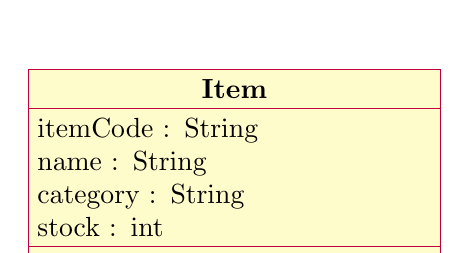
\begin{tikzpicture}
            \begin{class}[text width=5cm]{Item}{0,0}
                \attribute{itemCode : String}
                \attribute{name : String}
                \attribute{category : String}
                \attribute{stock : int}
            \end{class}
        \end{tikzpicture}
    }
    \item {
        \texttt{ItemService.java}
    
        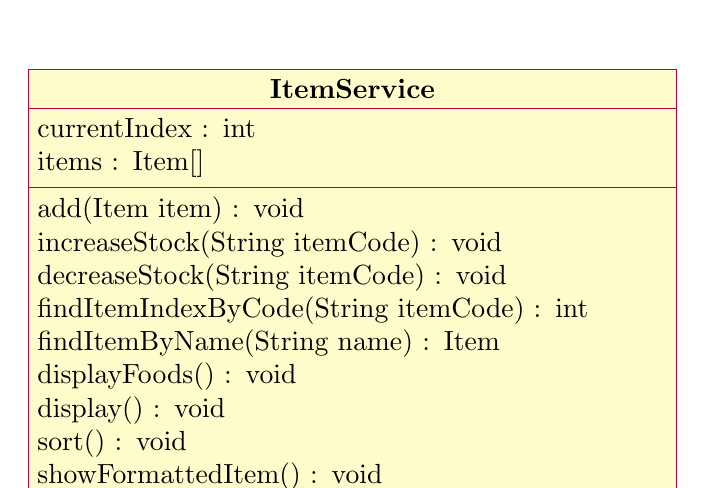
\begin{tikzpicture}
            \begin{class}[text width=8cm]{ItemService}{0,0}
                \attribute{currentIndex : int}
                \attribute{items : Item[]}
                \operation{add(Item item) : void}
                \operation{increaseStock(String itemCode) : void}
                \operation{decreaseStock(String itemCode) : void}
                \operation{findItemIndexByCode(String itemCode) : int}
                \operation{findItemByName(String name) : Item}
                \operation{displayFoods() : void}
                \operation{display() : void}
                \operation{sort() : void}
                \operation{showFormattedItem() : void}
            \end{class}
        \end{tikzpicture}
    }
    \item {
        \texttt{Main.java}
    
        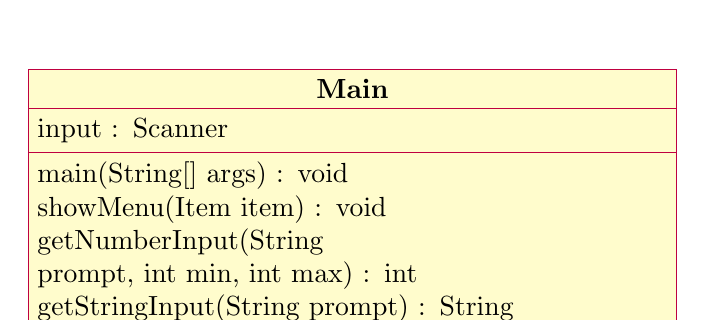
\begin{tikzpicture}
            \begin{class}[text width=8cm]{Main}{0,0}
                \attribute{input : Scanner}
                \operation{main(String[] args) : void}
                \operation{showMenu(Item item) : void}
                \operation{getNumberInput(String prompt, int min, int max) : int}
                \operation{getStringInput(String prompt) : String}
            \end{class}
        \end{tikzpicture}
    }
\end{itemize}

\pagebreak

\section{Code}
\begin{enumerate}
    \item {
        \textbf{Item.java}

        \begin{minted}[autogobble,linenos,fontsize=\small]{java}
        public class Item {
            String itemCode;
            String name;
            String category;
            int stock;

            public Item(String itemCode, String name, String category, int stock) {
                this.itemCode = itemCode;
                this.name = name;
                this.category = category;
                this.stock = stock;
            }
        }
        \end{minted}
    }
    \item {
        \textbf{ItemService.java}

        \begin{minted}[autogobble,linenos,fontsize=\small]{java}
        public class ItemService {
            private int currentIndex = -1;
            private final Item[] items = new Item[100];

            /**
             * Adds a new item to the storage
             * @param item The item you want to add
             */
            public void add(Item item) {
                if (currentIndex > items.length - 1) {
                    System.out.println(
                        "The storage is already full, " +
                        "please remove an item before adding a new one.");
                    return;
                }

                currentIndex++;
                items[currentIndex] = item;
            }

            /**
             * Adds the stock for certain item using the itemCode
             * @param itemCode The code of the item
             * @param stock The amount of stock
             */
            public void increaseStock(String itemCode, int stock) {
                int itemIndex = findItemIndexByCode(itemCode);
                if (itemIndex == -1) {
                    System.out.println("There is no item with an id of: " + itemCode);
                    return;
                }

                items[itemIndex].stock += stock;
            }

            /**
             * Adds the stock for certain item using the itemCode
             * @param itemCode The code of the item
             * @param stock The amount of stock
             */
            public void decreaseStock(String itemCode, int stock) {
                int itemIndex = findItemIndexByCode(itemCode);
                if (itemIndex == -1) {
                    System.out.println("There is no item with an id of: " + itemCode);
                    return;
                }

                items[itemIndex].stock -= stock;
            }

            /**
             * Finds an item index based on its item code
             * @param itemCode The code of the item you want to find
             * @return The item index if found, -1 if not found
             */
            public int findItemIndexByCode(String itemCode) {
                for (int i = 0; i < currentIndex; i++) {
                    if (items[i].itemCode.equals(itemCode)) {
                        return i;
                    }
                }
                return -1;
            }

            /**
             * Finds an item based on its name. This method is case insensitive
             * @param name The name of the item
             * @return The matching item, null if not found
             */
            public Item findItemByName(String name) {
                for (int i = 0; i < currentIndex; i++) {
                    if (items[i].name.equalsIgnoreCase(name)) {
                        return items[i];
                    }
                }
                return null;
            }

            /**
             * Displays every items that has a category of 'food'. Case insensitive
             */
             public void displayFoodsWithNoStock() {
                for (int i = 0; i < currentIndex; i++) {
                    Item currentItem = items[i];
                    if (!currentItem.category.equalsIgnoreCase("food")
                            && currentItem.stock > 0) continue;
                    showFormattedItem(currentItem);
                }
            }

            /**
             * Display all items
             */
            public void display() {
                for (int i = 0; i < currentIndex; i++) {
                    Item currentItem = items[i];
                    showFormattedItem(currentItem);
                }
            }

            /**
             * Sorts the items using bubble sort algorithm based on its stock (ascending)
             */
            public void sort() {
                for (int i = 0; i < currentIndex - 1; i++) {
                    for (int j = 1; j < currentIndex - i; j++) {
                        if (items[j].stock < items[j - 1].stock) {
                            Item tmp = items[j];
                            items[j] = items[j - 1];
                            items[j - 1] = tmp;
                        }
                    }
                }
            }

            /**
             * Shows the item using predefined format to stdout
             * @param item The item you want to show
             */
            public void showFormattedItem(Item item) {
                System.out.println("------------------");
                System.out.println("Item Code\t: " + item.itemCode);
                System.out.println("Name\t\t: " + item.name);
                System.out.println("Category\t: " + item.category);
                System.out.println("Stock\t\t: " + item.stock);
                System.out.println("------------------");
            }
        }
        \end{minted}
    }
    \item {
        \textbf{Main.java}

        \begin{minted}[autogobble,linenos,fontsize=\small]{java}
        public class Main {
            private static Scanner input = new Scanner(System.in);

            public static void main(String[] args) {
                Item[] items = {
                        new Item("16030927", "Indomilk", "drink", 100),
                        new Item("16100617", "Sprite", "drink", 70),
                        new Item("16240401", "Yakult", "drink", 500),
                        new Item("16270525", "Indomie", "food", 250),
                        new Item("16971204", "Oreo", "food", 320),
                        new Item("16100727", "Chocochips", "food", 120),
                        new Item("16460329", "Ballpoint", "stationary", 75),
                        new Item("16320421", "Pencil", "stationary", 110),
                        new Item("16180729", "Book", "stationary", 57),
                };
                ItemService itemService = new ItemService();

                // seed with initial data
                for (Item item : items) {
                    itemService.add(item);
                }

                // loop indefinitely until the user wants to stop
                while (true) {
                    showMenu();
                    int chosenMenu = getNumberInput("Choose Menu: ", 1, 7);
                    switch (chosenMenu) {
                        case 1: {
                            String itemCode = getStringInput("Insert the item code: ");
                            String name = getStringInput("Insert the name: ");
                            String category = getStringInput("Insert the category: ");
                            int stock = getNumberInput("Insert the initial stock: ", 1, 1000);
                            itemService.add(new Item(itemCode, name, category, stock));
                            System.out.println("New item has been successfully added");
                            break;
                        }
                        case 2: {
                            itemService.display();
                            break;
                        }
                        case 3: {
                            itemService.sort();
                            System.out.println(
                                    "Items has been sorted based on" +
                                            " its stock value (ascending)"
                            );
                            break;
                        }
                        case 4: {
                            itemService.displayFoodsWithNoStock();
                            break;
                        }
                        case 5: {
                            String name = getStringInput("Insert the food name: ");
                            Item item = itemService.findItemByName(name);
                            if (item == null) {
                                System.out.println(
                                        "The item was not found. " +
                                        "Try with other name instead.");
                                break;
                            }
                            itemService.showFormattedItem(item);
                            break;
                        }
                        case 6: {
                            String itemCode = getStringInput("Insert the item code: ");
                            int stock = getNumberInput(
                                    "Insert the stock you want to add: ", 
                                    1, 1000
                            );
                            itemService.increaseStock(itemCode, stock);
                            System.out.println(
                                    "Stock has been added to an item with an ID of: "
                                    + itemCode
                            );
                            break;
                        }
                        case 7: {
                            String itemCode = getStringInput("Insert the item code: ");
                            int stock = getNumberInput(
                                    "Insert the stock you want to add: ", 
                                    1, 1000
                            );
                            itemService.decreaseStock(itemCode, stock);
                            System.out.println(
                                    "Stock has been added to an item with an ID of: "
                                    + itemCode
                            );
                            break;
                        }
                        default: {
                            System.out.println("Incorrect choice, please try again!");
                        }
                    }

                    // break from the loop if the user no longer wants to continue
                    String shouldContinueAnswer = getStringInput(
                            "Do you want to continue (y/n)? "
                    );
                    if (!shouldContinueAnswer.equalsIgnoreCase("y")) break;
                }
            }

            /**
             * Shows the available menu for the program
             */
            private static void showMenu() {
                String[] menu = {
                        "Add Item",
                        "Display All Items",
                        "Sort Items by Stock (Ascending)",
                        "Display All Foods with No Stock",
                        "Search Item by Name",
                        "Add Stock for Item",
                        "Decrease Stock for Item",
                };
                System.out.println("== Stock Management Program == ");
                for (int i = 0; i < menu.length; i++) {
                    System.out.printf("%d. %s\n", i + 1, menu[i]);
                }
            }

            /**
             * Shortcut to get a user input in form of int
             * @param prompt The prompt to show to the user
             * @param min The minimum valid amount
             * @param max The maximum valid amount
             * @return The answer in integer within the specified bound
             */
            private static int getNumberInput(String prompt, int min, int max) {
                while (true) {
                    System.out.print(prompt);
                    int answer = input.nextInt();
                    // consumes the next newline
                    input.nextLine();
                    if (answer >= min && answer <= max) return answer;
                    System.out.printf("The input can only be between %d and %d.", min, max);
                }
            }

            /**
             * Shortcut to get a user input in form of String
             * @param prompt The prompt to show to the user
             * @return The answer as a string
             */
            private static String getStringInput(String prompt) {
                System.out.print(prompt);
                return input.nextLine();
            }
        }
        \end{minted}
    }
\end{enumerate}



\end{document}

